% !TEX root = ./Incompressible_Flow_over_Airfoils.tex

\tikzset{every picture/.style={line width=0.75pt}} %set default line width to 0.75pt        

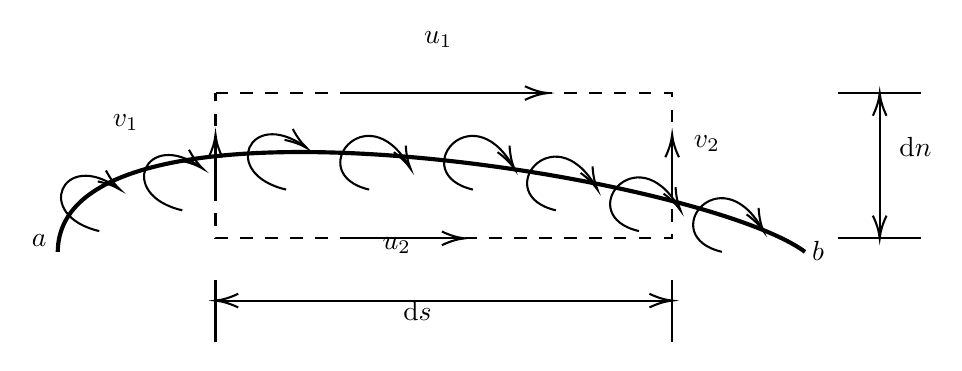
\begin{tikzpicture}[x=0.75pt,y=0.75pt,yscale=-1,xscale=1]
%uncomment if require: \path (0,285); %set diagram left start at 0, and has height of 285

%Curve Lines [id:da8763652678817189] 
\draw [line width=1.5]    (104,206.5) .. controls (104.51,119.91) and (414,169.5) .. (464,206.5) ;
%Curve Lines [id:da4750021580535706] 
\draw    (124,196.5) .. controls (92,189.03) and (106.07,156.9) .. (132.77,175.61) ;
\draw [shift={(134,176.5)}, rotate = 216.83] [color={rgb, 255:red, 0; green, 0; blue, 0 }  ][line width=0.75]    (10.93,-3.29) .. controls (6.95,-1.4) and (3.31,-0.3) .. (0,0) .. controls (3.31,0.3) and (6.95,1.4) .. (10.93,3.29)   ;
%Curve Lines [id:da2895808384347458] 
\draw    (164,186.5) .. controls (132,179.03) and (146.07,146.9) .. (172.77,165.61) ;
\draw [shift={(174,166.5)}, rotate = 216.83] [color={rgb, 255:red, 0; green, 0; blue, 0 }  ][line width=0.75]    (10.93,-3.29) .. controls (6.95,-1.4) and (3.31,-0.3) .. (0,0) .. controls (3.31,0.3) and (6.95,1.4) .. (10.93,3.29)   ;
%Curve Lines [id:da7153231460572151] 
\draw    (214,176.5) .. controls (182,169.03) and (196.07,136.9) .. (222.77,155.61) ;
\draw [shift={(224,156.5)}, rotate = 216.83] [color={rgb, 255:red, 0; green, 0; blue, 0 }  ][line width=0.75]    (10.93,-3.29) .. controls (6.95,-1.4) and (3.31,-0.3) .. (0,0) .. controls (3.31,0.3) and (6.95,1.4) .. (10.93,3.29)   ;
%Curve Lines [id:da9877697377632966] 
\draw    (254,176.5) .. controls (222,169.03) and (252.56,130.11) .. (273.07,164.86) ;
\draw [shift={(274,166.5)}, rotate = 241.4] [color={rgb, 255:red, 0; green, 0; blue, 0 }  ][line width=0.75]    (10.93,-3.29) .. controls (6.95,-1.4) and (3.31,-0.3) .. (0,0) .. controls (3.31,0.3) and (6.95,1.4) .. (10.93,3.29)   ;
%Curve Lines [id:da6202187083118886] 
\draw    (304,176.5) .. controls (272,169.03) and (302.56,130.11) .. (323.07,164.86) ;
\draw [shift={(324,166.5)}, rotate = 241.4] [color={rgb, 255:red, 0; green, 0; blue, 0 }  ][line width=0.75]    (10.93,-3.29) .. controls (6.95,-1.4) and (3.31,-0.3) .. (0,0) .. controls (3.31,0.3) and (6.95,1.4) .. (10.93,3.29)   ;
%Curve Lines [id:da8336758488674814] 
\draw    (344,186.5) .. controls (312,179.03) and (342.56,140.11) .. (363.07,174.86) ;
\draw [shift={(364,176.5)}, rotate = 241.4] [color={rgb, 255:red, 0; green, 0; blue, 0 }  ][line width=0.75]    (10.93,-3.29) .. controls (6.95,-1.4) and (3.31,-0.3) .. (0,0) .. controls (3.31,0.3) and (6.95,1.4) .. (10.93,3.29)   ;
%Curve Lines [id:da8897778956265143] 
\draw    (384,196.5) .. controls (352,189.03) and (382.56,150.11) .. (403.07,184.86) ;
\draw [shift={(404,186.5)}, rotate = 241.4] [color={rgb, 255:red, 0; green, 0; blue, 0 }  ][line width=0.75]    (10.93,-3.29) .. controls (6.95,-1.4) and (3.31,-0.3) .. (0,0) .. controls (3.31,0.3) and (6.95,1.4) .. (10.93,3.29)   ;
%Curve Lines [id:da04487167241342771] 
\draw    (424,206.5) .. controls (392,199.03) and (422.56,160.11) .. (443.07,194.86) ;
\draw [shift={(444,196.5)}, rotate = 241.4] [color={rgb, 255:red, 0; green, 0; blue, 0 }  ][line width=0.75]    (10.93,-3.29) .. controls (6.95,-1.4) and (3.31,-0.3) .. (0,0) .. controls (3.31,0.3) and (6.95,1.4) .. (10.93,3.29)   ;
%Shape: Rectangle [id:dp15963879701718064] 
\draw  [dash pattern={on 4.5pt off 4.5pt}] (180,130) -- (400,130) -- (400,200) -- (180,200) -- cycle ;
%Straight Lines [id:da8026280446997687] 
\draw    (240,130) -- (338,130) ;
\draw [shift={(340,130)}, rotate = 180] [color={rgb, 255:red, 0; green, 0; blue, 0 }  ][line width=0.75]    (10.93,-3.29) .. controls (6.95,-1.4) and (3.31,-0.3) .. (0,0) .. controls (3.31,0.3) and (6.95,1.4) .. (10.93,3.29)   ;
%Straight Lines [id:da3245350317643181] 
\draw    (240,200) -- (298,200) ;
\draw [shift={(300,200)}, rotate = 180] [color={rgb, 255:red, 0; green, 0; blue, 0 }  ][line width=0.75]    (10.93,-3.29) .. controls (6.95,-1.4) and (3.31,-0.3) .. (0,0) .. controls (3.31,0.3) and (6.95,1.4) .. (10.93,3.29)   ;
%Straight Lines [id:da7628086801385121] 
\draw    (180,180) -- (180,152) ;
\draw [shift={(180,150)}, rotate = 90] [color={rgb, 255:red, 0; green, 0; blue, 0 }  ][line width=0.75]    (10.93,-3.29) .. controls (6.95,-1.4) and (3.31,-0.3) .. (0,0) .. controls (3.31,0.3) and (6.95,1.4) .. (10.93,3.29)   ;
%Straight Lines [id:da347003095117139] 
\draw    (400,180) -- (400,152) ;
\draw [shift={(400,150)}, rotate = 90] [color={rgb, 255:red, 0; green, 0; blue, 0 }  ][line width=0.75]    (10.93,-3.29) .. controls (6.95,-1.4) and (3.31,-0.3) .. (0,0) .. controls (3.31,0.3) and (6.95,1.4) .. (10.93,3.29)   ;
%Straight Lines [id:da6243635216764141] 
\draw    (180,220) -- (180,250) ;
%Straight Lines [id:da6817985927803263] 
\draw    (400,220) -- (400,250) ;
%Straight Lines [id:da9105574441608693] 
\draw    (290,230) -- (398,230) ;
\draw [shift={(400,230)}, rotate = 180] [color={rgb, 255:red, 0; green, 0; blue, 0 }  ][line width=0.75]    (10.93,-3.29) .. controls (6.95,-1.4) and (3.31,-0.3) .. (0,0) .. controls (3.31,0.3) and (6.95,1.4) .. (10.93,3.29)   ;
%Straight Lines [id:da7767579818993569] 
\draw    (290,230) -- (182,230) ;
\draw [shift={(180,230)}, rotate = 360] [color={rgb, 255:red, 0; green, 0; blue, 0 }  ][line width=0.75]    (10.93,-3.29) .. controls (6.95,-1.4) and (3.31,-0.3) .. (0,0) .. controls (3.31,0.3) and (6.95,1.4) .. (10.93,3.29)   ;
%Straight Lines [id:da3361994371134467] 
\draw    (480,200) -- (520,200) ;
%Straight Lines [id:da04570162822709278] 
\draw    (480,130) -- (520,130) ;
%Straight Lines [id:da6631521119255424] 
\draw    (500,160) -- (500,198) ;
\draw [shift={(500,200)}, rotate = 270] [color={rgb, 255:red, 0; green, 0; blue, 0 }  ][line width=0.75]    (10.93,-3.29) .. controls (6.95,-1.4) and (3.31,-0.3) .. (0,0) .. controls (3.31,0.3) and (6.95,1.4) .. (10.93,3.29)   ;
%Straight Lines [id:da14321333492030197] 
\draw    (500,160) -- (500,132) ;
\draw [shift={(500,130)}, rotate = 90] [color={rgb, 255:red, 0; green, 0; blue, 0 }  ][line width=0.75]    (10.93,-3.29) .. controls (6.95,-1.4) and (3.31,-0.3) .. (0,0) .. controls (3.31,0.3) and (6.95,1.4) .. (10.93,3.29)   ;

% Text Node
\draw (90,196.5) node [anchor=north west][inner sep=0.75pt]    {$a$};
% Text Node
\draw (466,200) node [anchor=north west][inner sep=0.75pt]    {$b$};
% Text Node
\draw (279,99) node [anchor=north west][inner sep=0.75pt]    {$u_{1}$};
% Text Node
\draw (259,198) node [anchor=north west][inner sep=0.75pt]    {$u_{2}$};
% Text Node
\draw (129,139) node [anchor=north west][inner sep=0.75pt]    {$v_{1}$};
% Text Node
\draw (409,149) node [anchor=north west][inner sep=0.75pt]    {$v_{2}$};
% Text Node
\draw (269,229) node [anchor=north west][inner sep=0.75pt]    {$\mathrm{d}s$};
% Text Node
\draw (508,150) node [anchor=north west][inner sep=0.75pt]    {$\mathrm{d}n$};


\end{tikzpicture}
